\documentclass[a4paper,oneside,12pt]{report}
\usepackage{fontspec}
\usepackage{setspace}
\usepackage{amsmath}
\usepackage{titling}
\usepackage{geometry}
\usepackage{listings}
\usepackage{xcolor}
\usepackage{float}
\usepackage{hyperref}
\usepackage{indentfirst}
\usepackage{url}
\usepackage{fancyhdr}
\usepackage{tocloft}
\usepackage{bookmark}
\usepackage{booktabs}
\usepackage{caption}
\usepackage{tikz}
\usetikzlibrary{positioning,shapes.geometric,arrows.meta,decorations.pathreplacing}

\setmainfont{texgyretermes-regular.otf}[
    BoldFont=texgyretermes-bold.otf,
    ItalicFont=texgyretermes-italic.otf,
    BoldItalicFont=texgyretermes-bolditalic.otf
]
\onehalfspacing
\geometry{left=3cm, right=2.5cm, top=2cm, bottom=2.5cm}
\sloppy

\definecolor{codegreen}{rgb}{0,0.6,0}
\definecolor{codegray}{rgb}{0.5,0.5,0.5}
\definecolor{codepurple}{rgb}{0.58,0,0.82}
\definecolor{backcolour}{rgb}{0.95,0.95,0.92}
\definecolor{darkblue}{rgb}{0,0,0.6}

\lstdefinestyle{commonstyle}{
    backgroundcolor=\color{backcolour},
    breakatwhitespace=false,
    breaklines=true,
    captionpos=b,
    keepspaces=true,
    numbers=left,
    numbersep=5pt,
    showspaces=false,
    showstringspaces=false,
    showtabs=false,
    tabsize=2,
    frame=single,
    basicstyle=\ttfamily\footnotesize,
    numberstyle=\tiny\color{codegray},
    columns=flexible,
    postbreak=\mbox{\textcolor{red}{$\hookrightarrow$}\space},
    breakindent=0pt,
    breakautoindent=false
}
\lstdefinestyle{bashstyle}{
    style=commonstyle,
    language=bash,
    commentstyle=\color{codegreen},
    keywordstyle=\color{darkblue},
    stringstyle=\color{codepurple}
}
\lstdefinestyle{yamlstyle}{
    style=commonstyle,
    commentstyle=\color{codegreen},
    keywordstyle=\color{darkblue},
    stringstyle=\color{codepurple}
}
\lstdefinestyle{dockerstyle}{
    style=commonstyle,
    commentstyle=\color{codegreen},
    keywordstyle=\color{darkblue},
    stringstyle=\color{codepurple}
}
\lstdefinestyle{phpstyle}{
    style=commonstyle,
    language=PHP,
    commentstyle=\color{codegreen},
    keywordstyle=\color{darkblue},
    stringstyle=\color{codepurple}
}

\newcommand{\customfbox}[1]{%
  \setlength{\fboxsep}{0pt}%
  \setlength{\fboxrule}{0.5pt}%
  \fcolorbox{black}{white}{#1}%
}

\renewcommand{\figurename}{Gambar}
\renewcommand{\thefigure}{\arabic{figure}}
\hypersetup{
    colorlinks=true,
    linkcolor=black,
    filecolor=black,
    urlcolor=black,
    citecolor=black,
    pdftitle={Laporan UTS Konstruksi dan Evolusi Perangkat Lunak},
    pdfpagemode=FullScreen,
    breaklinks=true
}
\pagestyle{fancy}
\fancyhf{}
\fancyfoot[C]{\thepage}
\renewcommand{\headrulewidth}{0pt}
\fancypagestyle{plain}{
    \fancyhf{}
    \fancyfoot[C]{\thepage}
    \renewcommand{\headrulewidth}{0pt}
}
\renewcommand{\contentsname}{Daftar Isi}
\renewcommand{\bibname}{Daftar Pustaka}
\renewcommand{\thechapter}{}
\renewcommand{\chaptername}{}
\renewcommand{\thesection}{\arabic{chapter}.\arabic{section}}
\renewcommand{\thesubsection}{\thesection.\arabic{subsection}}
\setcounter{secnumdepth}{3}
\setcounter{tocdepth}{3}
\renewcommand{\cftchapdotsep}{\cftdotsep}
\renewcommand{\cftchapleader}{\cftdotfill{\cftchapdotsep}}
\setlength{\cftchapindent}{0em}
\setlength{\cftsecindent}{2em}
\setlength{\cftsubsecindent}{4em}
\setlength{\cftchapnumwidth}{0em}
\setlength{\cftsecnumwidth}{2.5em}
\setlength{\cftsubsecnumwidth}{3.2em}
\renewcommand{\cftchappresnum}{}
\renewcommand{\cftchapaftersnum}{}

\begin{document}

\newgeometry{left=3cm, right=2.5cm, top=2.5cm, bottom=3cm}
\begin{titlingpage}
\begin{spacing}{1}
\begin{center}
\vspace*{0.2cm}
{\large \textbf{\MakeUppercase{Laporan Ujian Tengah Semester}}} \\[0.4cm]
{\large \textbf{\MakeUppercase{Konstruksi dan Evolusi Perangkat Lunak}}} \\[0.4cm]
{\large \textbf{\MakeUppercase{Sistem Manajemen Aset Laboratorium dengan CI/CD dan Containerization}}} \\[1.3cm]


\includegraphics[height=6.5cm]{images/UGM.png} \\[0.7cm]

{\normalsize \textbf{Disusun oleh:}} \\[0.4cm]
\begin{tabular}{@{}l l @{}}
  \textbf{Nama}           & : Hafidz Rizqullah Prasetya \\
  \textbf{NIM}            & : 24/535493/SV/24243 \\
  \textbf{Kelas}          & : PL5A1 \\
  \textbf{Dosen Pengampu} & : Dr. Muhammad Fakhrurrifqi, S.Kom., M.Cs. \\
                          & \hphantom{:} Galih Malela Damaraji, S.Pd., M.Eng. \\
\end{tabular} \\[1.1cm]

{\normalsize \textbf{PROGRAM STUDI D-IV}} \\[0.2cm]
{\normalsize \textbf{TEKNOLOGI REKAYASA PERANGKAT LUNAK}} \\[0.2cm]
{\normalsize \textbf{DEPARTEMEN TEKNIK ELEKTRO DAN INFORMATIKA}} \\[0.2cm]
{\normalsize \textbf{SEKOLAH VOKASI}} \\[0.2cm]
{\normalsize \textbf{UNIVERSITAS GADJAH MADA}} \\[0.2cm]
{\normalsize \textbf{YOGYAKARTA}} \\[0.2cm]
{\normalsize \textbf{2026}} \\[1.0cm]
\end{center}
\end{spacing}
\end{titlingpage}
\restoregeometry

\thispagestyle{empty}
\pagenumbering{roman}
\setcounter{page}{1}

\tableofcontents
\newpage

\pagenumbering{arabic}
\setcounter{page}{1}

\chapter{BAB I\\PENDAHULUAN}
\renewcommand{\thechapter}{1}

\section{Latar Belakang}
Pengembangan perangkat lunak modern menuntut integrasi yang solid antara arsitektur aplikasi dan siklus operasional pengembangan. Pendekatan tradisional yang memisahkan tahap pemrograman dengan tahap pengujian serta penerapan ke lingkungan produksi sering memicu inkonsistensi lingkungan, kegagalan integrasi, dan keterlambatan rilis. Konsep DevOps dan filosofi \textit{agile} hadir untuk menjembatani kesenjangan tersebut melalui otomatisasi alur kerja, pengujian berkelanjutan, dan standarisasi lingkungan eksekusi berbasis kontainer.

Dalam konteks rekayasa sistem terdistribusi, pemisahan tanggung jawab antara sisi penyedia data (\textit{backend}) dan antarmuka interaktif (\textit{frontend}) merupakan standar industri. Sisi \textit{backend} bertindak sebagai penyedia layanan RESTful API dengan protokol autentikasi berbasis token yang aman, sementara \textit{frontend} berfokus pada pengalaman pengguna yang dinamis dan modular. Untuk menjamin keandalan sistem berskala produksi, seluruh kode sumber dikelola menggunakan sistem kendali versi Git dengan aturan proteksi cabang yang ketat, diverifikasi melalui saluran integrasi berkelanjutan (\textit{Continuous Integration}), dan didistribusikan secara otomatis (\textit{Continuous Deployment}) ke dalam registri kontainer seperti GitHub Container Registry (GHCR).

\section{Tujuan Ujian}
Tujuan pengerjaan Ujian Tengah Semester mata kuliah Konstruksi dan Evolusi Perangkat Lunak ini mencakup pencapaian kompetensi pada beberapa Capaian Pembelajaran Mata Kuliah (CPMK):
\begin{enumerate}
    \item Menerapkan konsep dasar RESTful API, autentikasi berbasis token (Laravel Sanctum), dan antarmuka web modern (Vue.js 3) yang membaca konfigurasi dinamis (CPMK 1).
    \item Menerapkan prinsip integrasi berkelanjutan (CI) dan manajemen repositori Git dengan aturan proteksi cabang dan verifikasi otomatis menggunakan GitHub Actions (CPMK 2).
    \item Menerapkan penerapan berkelanjutan (CD) untuk membangun dan mempublikasikan citra kontainer ke GHCR dengan proteksi rahasia menggunakan GitHub Secrets (CPMK 3).
    \item Membangun berkas konfigurasi \textit{Dockerfile} untuk \textit{backend} Laravel dengan optimasi \textit{layer caching} dependensi Composer (CPMK 4).
    \item Menerapkan teknik \textit{multi-stage build} pada \textit{Dockerfile frontend} Vue.js menggunakan peladen Nginx tanpa menyertakan berkas dependensi kerja (CPMK 5).
\end{enumerate}

\section{Batasan Masalah dan Lingkup Sistem}
Lingkup pengerjaan ujian ini dibatasi pada perancangan dan implementasi Sistem Manajemen Inventaris Aset Laboratorium TRPL Sekolah Vokasi UGM. Sistem terdiri dari dua komponen utama:
\begin{enumerate}
    \item \textbf{Backend:} Layanan berbasis Laravel dengan basis data SQLite, autentikasi token Sanctum, proteksi seluruh rute privat, respons JSON baku (status 200, 201, 401, 422), dan pengujian otomatis \textit{feature test}.
    \item \textbf{Frontend:} Aplikasi berbasis Vue.js 3 dan Axios dengan halaman masuk pengguna, dasbor metrik aset, tabel inventaris, modal formulir penambahan dan pengubahan, serta penghapusan data dengan konfirmasi.
\end{enumerate}

\chapter{BAB II\\DASAR TEORI}
\renewcommand{\thechapter}{2}

\section{Arsitektur RESTful API dan Autentikasi Token}
REST (\textit{Representational State Transfer}) merupakan gaya arsitektur komunikasi data yang memanfaatkan metode standar protokol HTTP, seperti GET, POST, PUT, dan DELETE. Setiap operasi mencerminkan manipulasi keadaan sumber daya (\textit{resource}). Pada sistem RESTful yang stateless, peladen tidak menyimpan sesi pengguna di memori sisi server, melainkan memverifikasi setiap permintaan melalui token kriptografis pada tajuk HTTP \textit{Authorization} \cite{laravel-sanctum}.

Laravel Sanctum menyediakan mekanisme penerbitan token akses pribadi (\textit{Personal Access Token}) yang ringan. Ketika pengguna berhasil melakukan autentikasi, peladen menghasilkan string acak terenkripsi yang disimpan dalam basis data. Klien menyimpan token ini dan melampirkannya dengan skema \textit{Bearer Token} pada setiap permintaan ke endpoint terproteksi. Standarisasi respons HTTP menjadi indikator kepatuhan API, seperti status 201 untuk entitas baru, status 422 jika terjadi kegagalan validasi masukan, dan status 401 jika permintaan tidak menyertakan token yang sah \cite{laravel-sanctum}.

\section{Framework Frontend Reaktif dan Klien HTTP}
Vue.js adalah kerangka kerja JavaScript progresif yang mengadopsi pola arsitektur berbasis komponen reaktif. Melalui Composition API, status aplikasi dipantau secara otomatis sehingga perubahan data langsung direfleksikan pada antarmuka pengguna tanpa memuat ulang peramban \cite{vuejs}.

Komunikasi antara antarmuka Vue dan peladen API dijembatani oleh pustaka Axios. Axios mempermudah interceptor tajuk permintaan (\textit{request interceptor}) untuk menyisipkan token secara konsisten, serta menangani kegagalan autentikasi (\textit{response interceptor}) untuk membersihkan penyimpanan lokal saat token kedaluwarsa. Praktik rekayasa yang baik mengharuskan URL peladen dibaca dari variabel lingkungan (\textit{environment variable}) melalui Vite, sehingga kode sumber tidak terikat pada alamat jaringan tertentu \cite{axios}.

\section{Manajemen Repositori Git dan Proteksi Cabang}
Dalam alur kerja kolaboratif, cabang \texttt{main} diposisikan sebagai representasi kode produksi yang stabil, sedangkan cabang \texttt{dev} berfungsi sebagai wadah integrasi awal. Penambahan kapabilitas baru diisolasi pada cabang fitur (\textit{feature branch}) dan hanya dapat digabungkan ke cabang utama melalui mekanisme \textit{Pull Request} (PR) \cite{github-protection}.

Fitur \textit{Branch Protection Rules} di GitHub memungkinkan penegakan kebijakan keselamatan kode. Aturan ini melarang pengunggahan langsung (\textit{direct push}) dan mewajibkan seluruh pengujian otomatis (\textit{status checks}) berstatus lulus sebelum perubahan diizinkan untuk digabungkan. Pendekatan ini meminimalkan risiko regresi dan memastikan integritas basis kode tetap terjaga \cite{github-protection}.

\section{Otomatisasi Alur Kerja dengan GitHub Actions}
GitHub Actions adalah platform integrasi dan penerapan berkelanjutan terkelola yang mengeksekusi serangkaian pekerjaan (\textit{jobs}) berdasarkan kejadian tertentu pada repositori (\textit{triggers}). Alur kerja didefinisikan dalam format YAML di direktori \texttt{.github/workflows/} \cite{github-actions}.

Pemisahan pekerjaan antara pengujian sisi server (\textit{backend test}) dan kompilasi sisi klien (\textit{frontend build}) memungkinkan eksekusi secara paralel guna mempercepat umpan balik. Pada tahap lanjutan, pekerjaan penerapan (\textit{deploy job}) diatur agar hanya aktif ketika commit berhasil digabungkan ke cabang \texttt{main}, sedangkan pada cabang lain alur kerja otomatis berhenti setelah pengujian selesai \cite{github-actions}.

\section{Kontainerisasi dan Optimasi Dockerfile Multi-Stage}
Docker mengemas aplikasi beserta pustaka dan lingkungan dependensinya ke dalam satu unit mandiri yang disebut kontainer. Mekanisme ini menjamin bahwa aplikasi berjalan dengan perilaku yang identik di mesin pengembang, peladen CI, maupun peladen produksi \cite{docker-multistage}.

Penyusunan berkas \textit{Dockerfile} yang optimal memanfaatkan urutan lapisan instruksi (\textit{layer caching}). Dengan menyalin manifes dependensi (seperti \texttt{composer.json} dan \texttt{package.json}) sebelum kode sumber aplikasi, proses unduhan pustaka tidak perlu diulang jika kode sumber mengalami revisi. Pada aplikasi sisi klien, teknik \textit{multi-stage build} memisahkan lingkungan kompilasi berbasis Node.js dengan lingkungan eksekusi berbasis web server Nginx berukuran ringkas, sehingga berkas sementara dan pustaka pengembang tidak ikut terbawa ke citra akhir \cite{docker-multistage,nginx}.

\chapter{BAB III\\HASIL DAN PEMBAHASAN}
\renewcommand{\thechapter}{3}

\section{Backend Laravel RESTful API (CPMK 1)}
Pengerjaan soal nomor 1 difokuskan pada pembangunan layanan RESTful API menggunakan Laravel dengan tema Sistem Manajemen Aset Laboratorium. Sistem mengelola data inventaris perangkat keras dan instrumen yang digunakan dalam kegiatan praktikum di lingkungan kampus.

\subsection{Perancangan Skema Data dan Model}
Sumber daya utama yang dikelola adalah \texttt{Asset}. Tabel \texttt{assets} dirancang untuk menampung atribut kode inventaris unik, nama barang, kategori, status ketersediaan, nilai perolehan, dan lokasi laboratorium. Struktur migrasi basis data ditunjukkan pada Listing \ref{lst:migration-asset}.

\begin{lstlisting}[style=phpstyle,caption={Migrasi tabel assets pada backend Laravel.},label={lst:migration-asset}]
Schema::create('assets', function (Blueprint $table) {
    $table->id();
    $table->string('name');
    $table->string('code')->unique();
    $table->string('category');
    $table->string('status')->default('tersedia');
    $table->decimal('price', 15, 2);
    $table->string('location')->nullable();
    $table->timestamps();
});
\end{lstlisting}

Model \texttt{Asset} dilengkapi atribut pengisian massal (\textit{fillable}) untuk mencegah kerentanan \textit{mass assignment}, serta \textit{casting} tipe data desimal menjadi nilai numerik float pada respons JSON.

\subsection{Autentikasi Token Laravel Sanctum}
Autentikasi dikelola oleh \texttt{AuthController}. Pengguna melakukan autentikasi melalui rute publik \texttt{POST /api/login}. Jika alamat email dan kata sandi valid, peladen menghasilkan token teks biasa melalui metode \texttt{createToken()} dari trait \texttt{HasApiTokens}. Token tersebut dikirimkan kembali ke pengguna bersama informasi profil dasar.

Seluruh rute sumber daya dilindungi oleh middleware \texttt{auth:sanctum}. Jika pengguna mengirimkan permintaan tanpa menyertakan token atau menggunakan token yang sudah tidak berlaku, penanganan pengecualian pada \texttt{bootstrap/app.php} secara otomatis menangkap \texttt{AuthenticationException} dan mengembalikan respons JSON dengan status \textbf{401 Unauthorized}. Rute \texttt{POST /api/logout} mencabut token aktif pengguna sehingga token tersebut tidak dapat digunakan kembali.

\subsection{Implementasi Endpoint dan Status HTTP}
Operasi manipulasi data pada \texttt{AssetController} mengembalikan kode status HTTP standar sesuai ketentuan soal:
\begin{enumerate}
    \item \texttt{200 OK}: Dikembalikan saat pengambilan daftar aset (\texttt{GET /api/assets}), detail satu aset (\texttt{GET /api/assets/\{id\}}), pembaruan data (\texttt{PUT /api/assets/\{id\}}), dan penghapusan data (\texttt{DELETE /api/assets/\{id\}}).
    \item \texttt{201 Created}: Dikembalikan secara eksplisit saat penambahan entitas aset baru berhasil disimpan (\texttt{POST /api/assets}).
    \item \texttt{422 Unprocessable Content}: Dikembalikan oleh validator Laravel apabila masukan data tidak memenuhi aturan validasi (misalnya nama kosong, format harga bernilai negatif, atau kode aset sudah terdaftar).
    \item \texttt{401 Unauthorized}: Dikembalikan saat rute privat diakses tanpa menyertakan Bearer Token yang sah.
\end{enumerate}

\subsection{Koleksi Postman dan Pengujian Otomatis}
Seluruh endpoint diuji menggunakan koleksi Postman yang telah diekspor dan disimpan pada berkas \texttt{backend/postman/uts\_kepl\_asset\_api.postman\_collection.json}. Koleksi ini mencakup skrip uji otomatis yang menyimpan token sesi ke variabel koleksi secara instan setelah panggilan login berhasil.

Selain pengujian manual, keandalan sistem diverifikasi menggunakan pengujian unit dan fitur terotomatisasi (\textit{PHPUnit Feature Tests}) pada \texttt{tests/Feature/AuthApiTest.php} dan \texttt{tests/Feature/AssetApiTest.php}. Seluruh 13 pengujian dengan 47 penegasan (\textit{assertions}) berhasil diselesaikan dengan status lulus, sebagaimana ditunjukkan pada Gambar \ref{fig:feature-tests}.

\begin{figure}[H]
    \centering
    \customfbox{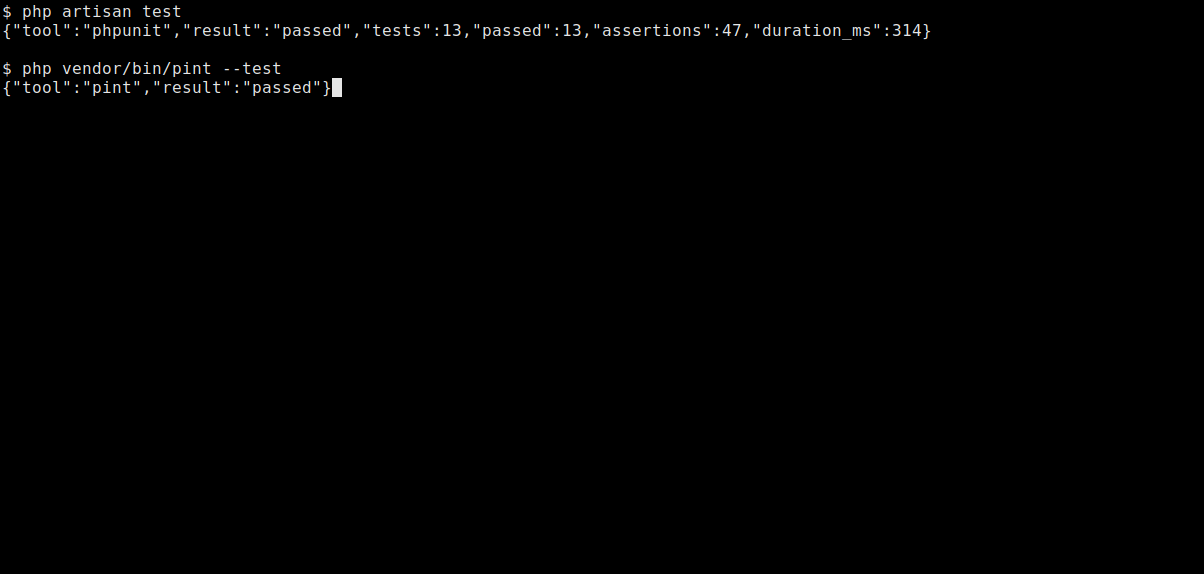
\includegraphics[width=0.95\textwidth]{images/ss-03-feature-tests.png}}
    \caption{Hasil eksekusi pengujian otomatis \texttt{php artisan test} dan pemeriksaan standar format kode \texttt{pint}.}
    \label{fig:feature-tests}
\end{figure}

Verifikasi kepatuhan kode status HTTP secara langsung melalui terminal ditampilkan pada Gambar \ref{fig:api-status-codes}, yang membuktikan bahwa respons kode 200, 201, 401, dan 422 bekerja secara konsisten.

\begin{figure}[H]
    \centering
    \customfbox{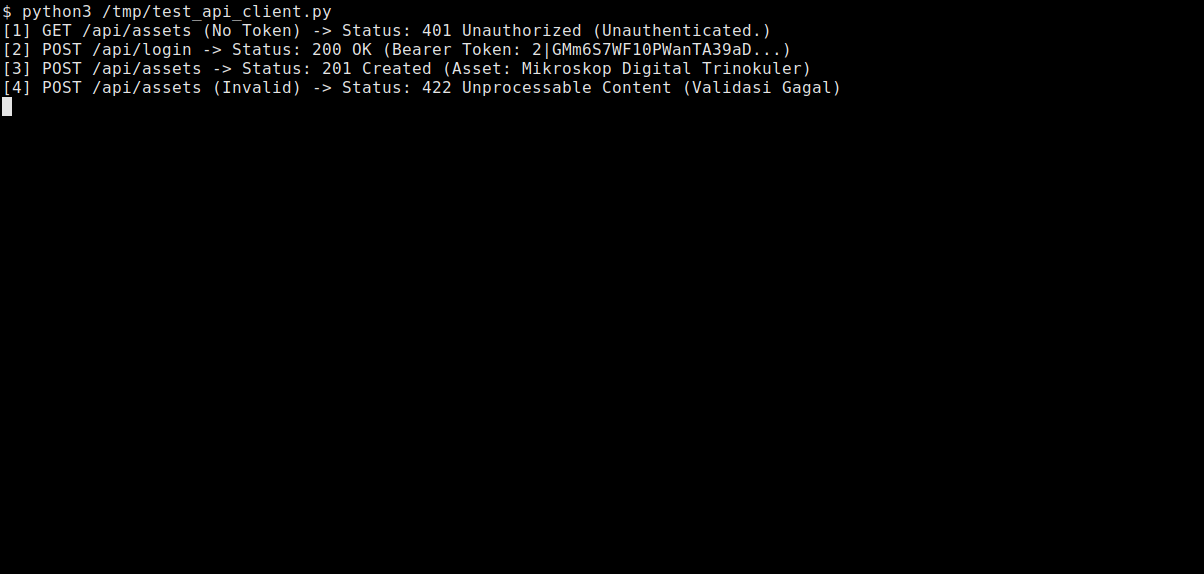
\includegraphics[width=0.95\textwidth]{images/ss-04-api-status-codes.png}}
    \caption{Verifikasi status code HTTP 401, 200, 201, dan 422 melalui pemanggilan klien API terminal.}
    \label{fig:api-status-codes}
\end{figure}

\section{Frontend Vue.js dan Axios (CPMK 1)}
Pengerjaan soal nomor 2 mencakup pembangunan antarmuka pengguna berbasis Vue.js 3 dengan bundler Vite dan pustaka HTTP Axios.

\subsection{Konfigurasi Variabel Lingkungan}
Untuk memenuhi ketentuan soal 2.c, alamat basis peladen API tidak ditulis mati di dalam kode komponen. Alamat dibaca dari berkas konfigurasi lingkungan \texttt{.env} melalui variabel \texttt{VITE\_API\_BASE\_URL}, seperti ditunjukkan pada Listing \ref{lst:vue-api-client}.

\begin{lstlisting}[style=bashstyle,caption={Konfigurasi klien Axios dengan pembacaan variabel lingkungan.},label={lst:vue-api-client}]
import axios from 'axios';

const apiBaseUrl = import.meta.env.VITE_API_BASE_URL || 'http://localhost:8000/api';

const apiClient = axios.create({
  baseURL: apiBaseUrl,
  headers: {
    'Accept': 'application/json',
    'Content-Type': 'application/json',
  },
});

apiClient.interceptors.request.use((config) => {
  const token = localStorage.getItem('auth_token');
  if (token) {
    config.headers.Authorization = `Bearer ${token}`;
  }
  return config;
});

export default apiClient;
\end{lstlisting}

\subsection{Antarmuka Masuk Pengguna dan Manajemen Token}
Ketika pengguna mengakses aplikasi untuk pertama kali, sistem menampilkan formulir masuk. Gambar \ref{fig:vue-login} memperlihatkan antarmuka halaman login yang menyertakan informasi alamat endpoint aktif yang dibaca dari variabel lingkungan.

\begin{figure}[H]
    \centering
    \customfbox{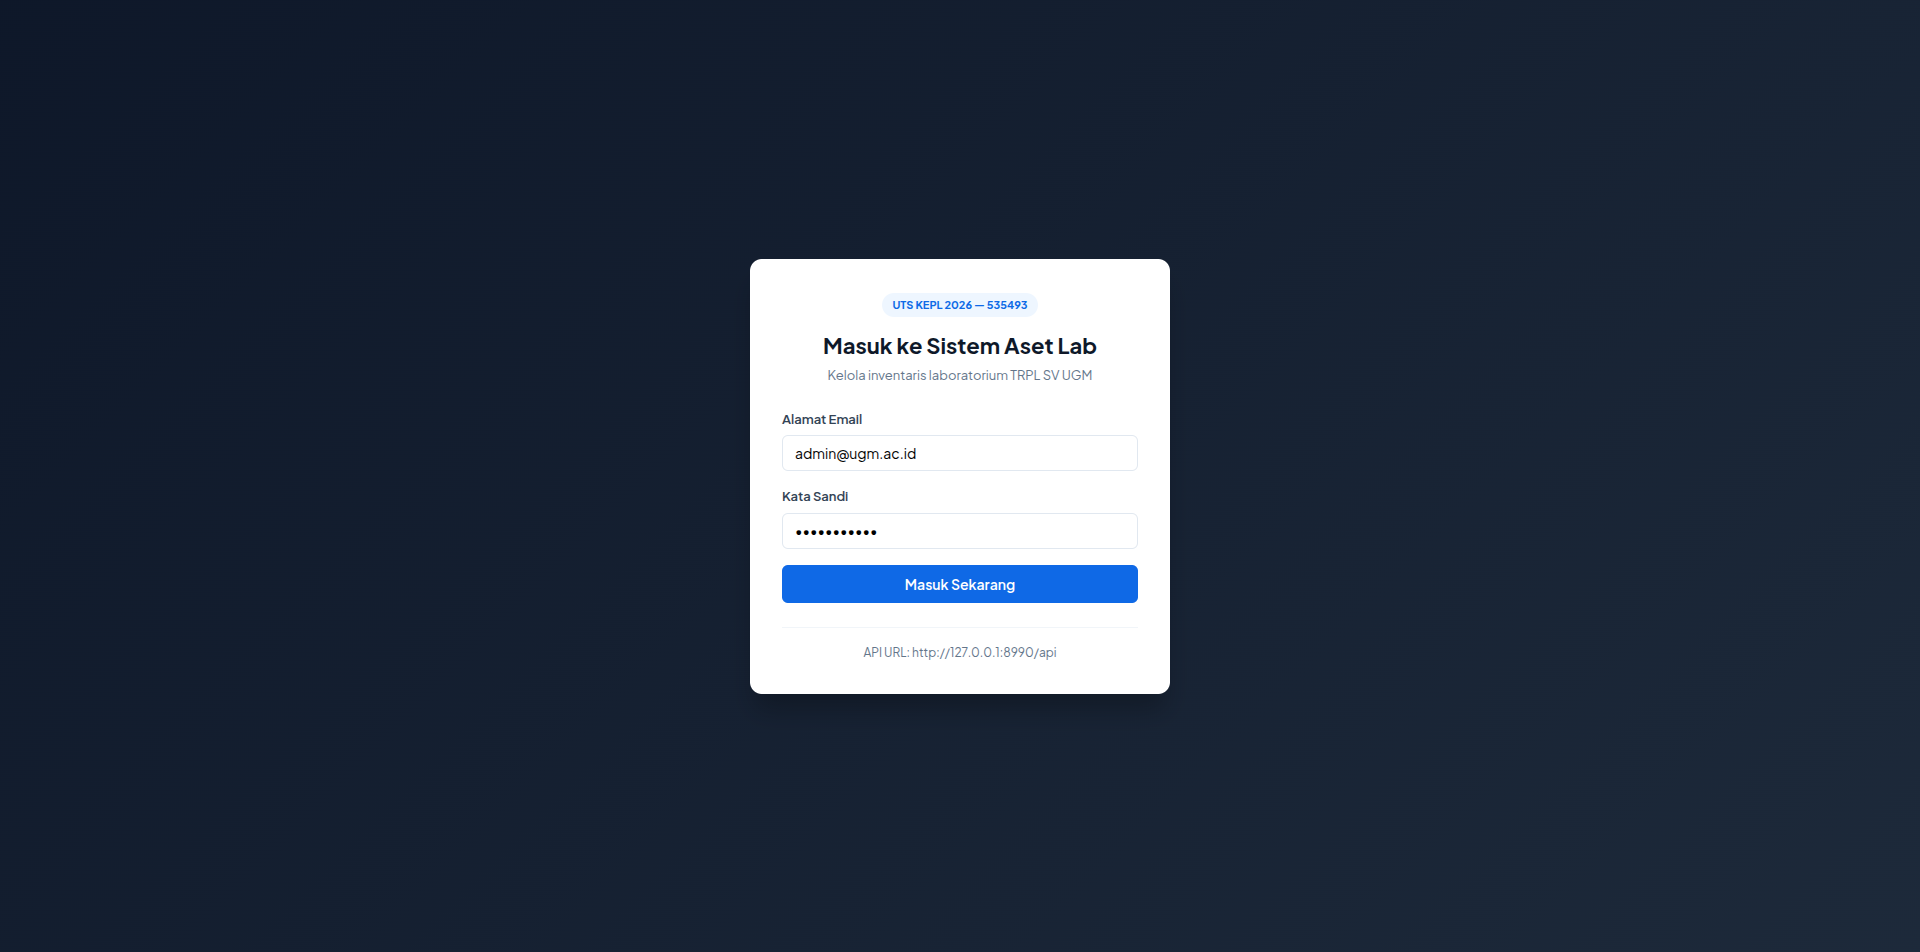
\includegraphics[width=0.95\textwidth]{images/ss-05a-vue-login.png}}
    \caption{Halaman login Vue.js dengan pembacaan konfigurasi variabel lingkungan API.}
    \label{fig:vue-login}
\end{figure}

Saat formulir dikirimkan, fungsi \texttt{handleLogin()} mengirim permintaan autentikasi ke backend. Token yang diterima disimpan ke dalam \texttt{localStorage} dengan kunci \texttt{auth\_token}. Berkat \textit{interceptor} Axios, token ini secara otomatis disertakan pada setiap permintaan HTTP berikutnya.

\subsection{Dasbor Metrik dan Pengelolaan Data Aset}
Setelah masuk, pengguna diarahkan ke antarmuka dasbor inventaris. Dasbor menampilkan ringkasan statistik (total aset, unit tersedia, unit dipinjam, dan total valuasi perolehan), fitur pencarian teks, penyaringan berdasarkan status, serta tabel inventaris lengkap. Tampilan dasbor disajikan pada Gambar \ref{fig:vue-dashboard}.

\begin{figure}[H]
    \centering
    \customfbox{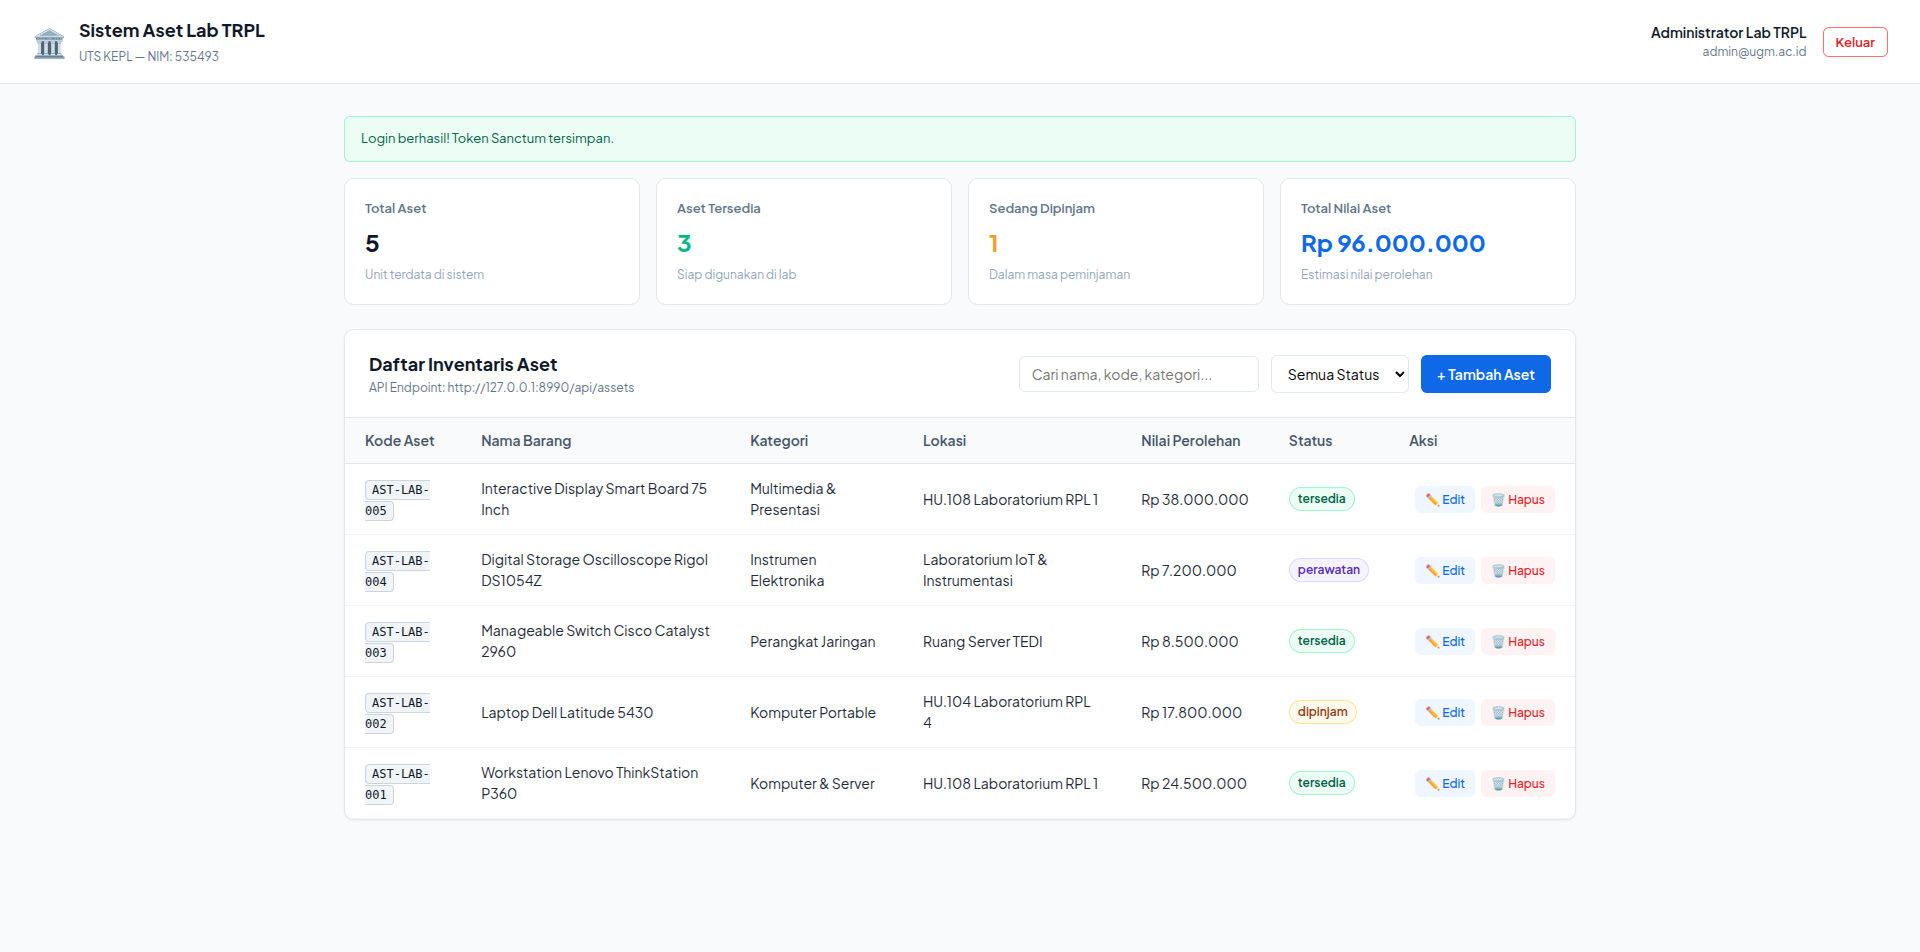
\includegraphics[width=0.95\textwidth]{images/ss-05b-vue-dashboard.png}}
    \caption{Dasbor manajemen inventaris aset laboratorium pada antarmuka Vue.js.}
    \label{fig:vue-dashboard}
\end{figure}

Penambahan aset baru dilakukan melalui jendela modal interaktif. Modal ini melakukan validasi masukan pada sisi klien sebelum mengirimkan data ke rute \texttt{POST /api/assets}. Apabila peladen mengembalikan kode 201 Created, daftar data pada tabel langsung diperbarui secara reaktif tanpa memuat ulang peramban. Tampilan modal penambahan aset ditunjukkan pada Gambar \ref{fig:vue-modal-tambah}.

\begin{figure}[H]
    \centering
    \customfbox{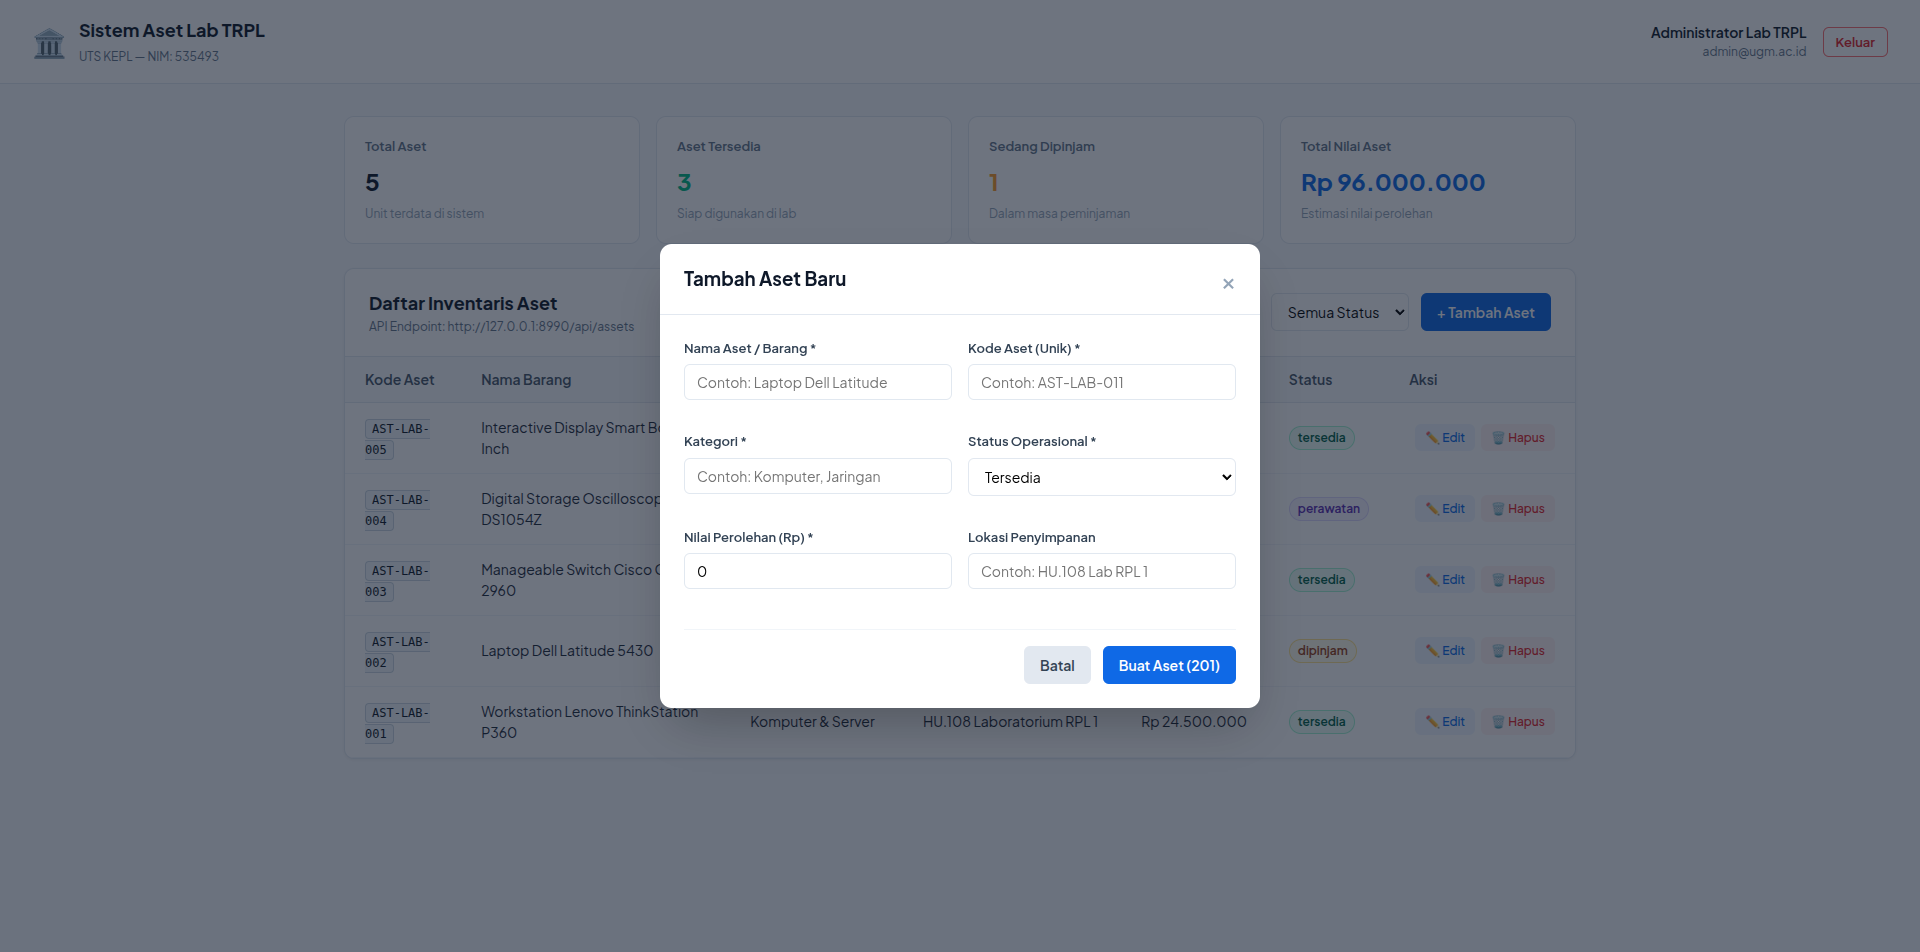
\includegraphics[width=0.95\textwidth]{images/ss-05c-vue-modal-tambah.png}}
    \caption{Modal interaktif penambahan aset laboratorium baru pada antarmuka frontend.}
    \label{fig:vue-modal-tambah}
\end{figure}

\section{Manajemen Repositori GitHub dan CI Pipeline (CPMK 2)}
Soal nomor 3 mewajibkan pengelolaan seluruh kode sistem pada repositori publik bernama \texttt{uts-p1-535493} di akun GitHub pribadi (\url{https://github.com/hafidzrizqullahprasetya/uts-p1-535493}), memuat folder \texttt{backend/} dan \texttt{frontend/}, serta menerapkan aturan cabang terlindungi.

\subsection{Struktur Repositori dan Strategi Percabangan}
Repositori diatur dengan tiga tingkatan cabang:
\begin{enumerate}
    \item \texttt{main}: Cabang produksi utama yang terlindungi secara ketat.
    \item \texttt{dev}: Cabang integrasi pengembangan pra-produksi.
    \item \texttt{feat/backend-and-frontend}: Cabang fitur yang menampung pengembangan awal kode backend, frontend, konfigurasi Docker, dan alur CI/CD.
\end{enumerate}

Seluruh perubahan kode dari cabang fitur diintegrasikan ke cabang \texttt{dev} melalui Pull Request nomor 1. Setelah diverifikasi lulus oleh pipa CI, cabang \texttt{dev} digabungkan ke cabang \texttt{main} melalui Pull Request nomor 2. Riwayat komit dan topologi pohon percabangan pada repositori ditampilkan pada Gambar \ref{fig:git-workflow}.

\begin{figure}[H]
    \centering
    \customfbox{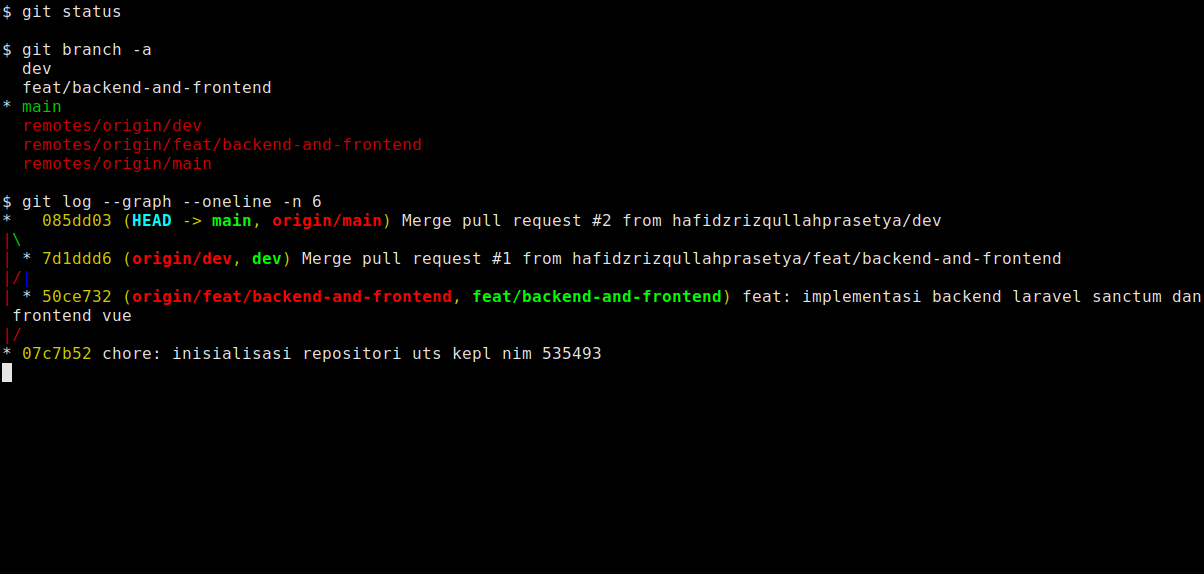
\includegraphics[width=0.95\textwidth]{images/ss-09-git-workflow.png}}
    \caption{Pemeriksaan status cabang Git lokal dan riwayat graf penggabungan Pull Request.}
    \label{fig:git-workflow}
\end{figure}

Tampilan beranda repositori publik di GitHub disajikan pada Gambar \ref{fig:repo-github}, yang memperlihatkan struktur direktori \texttt{backend/} dan \texttt{frontend/} yang bersih.

\begin{figure}[H]
    \centering
    \customfbox{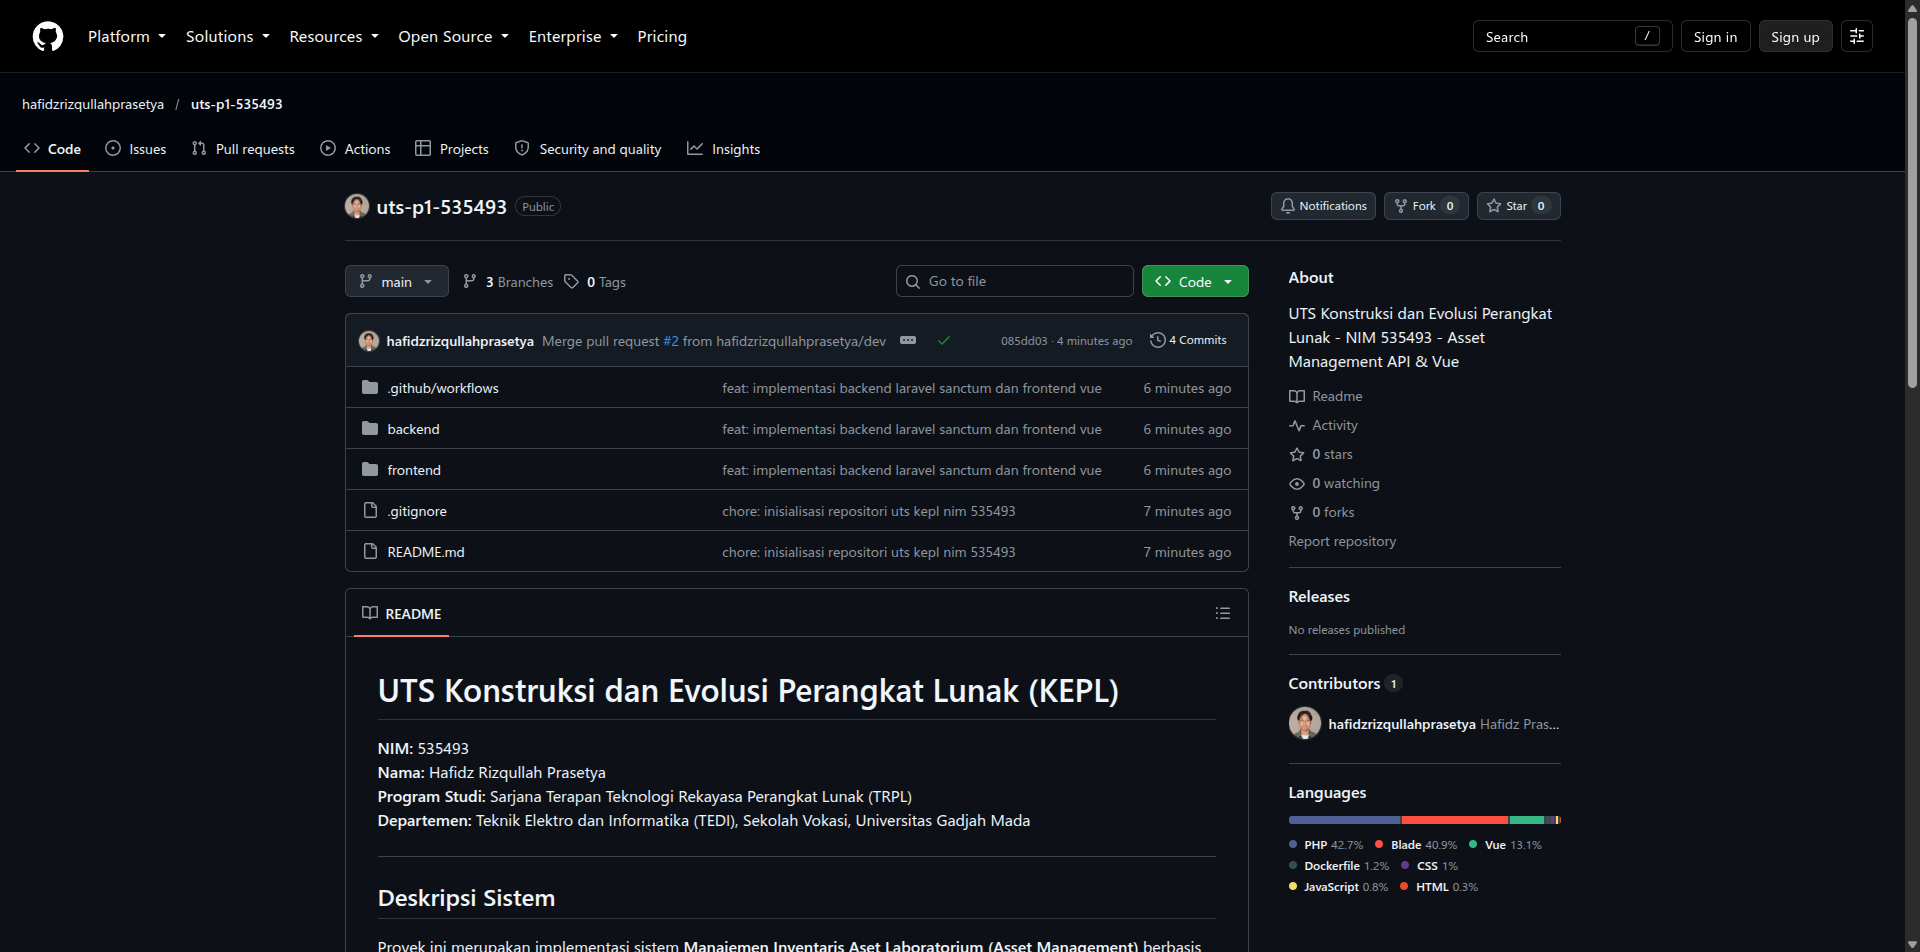
\includegraphics[width=0.95\textwidth]{images/ss-01-repo-github.png}}
    \caption{Tampilan repositori publik \texttt{uts-p1-535493} pada platform GitHub.}
    \label{fig:repo-github}
\end{figure}

\subsection{Konfigurasi Branch Protection Rules}
Sesuai instruksi soal, cabang \texttt{main} dan \texttt{dev} diproteksi untuk mencegah pengunggahan langsung (\textit{direct push}). Pengaturan proteksi cabang mewajibkan:
\begin{enumerate}
    \item Integrasi hanya dapat dilakukan melalui mekanisme Pull Request.
    \item Pemeriksaan status (\textit{status checks}) harus lulus sebelum penggabungan diizinkan, yaitu job \texttt{Backend Test} dan \texttt{Frontend Build}.
    \item Opsi cabang harus mutakhir (\textit{strict check: true}) sebelum digabungkan.
\end{enumerate}

Bukti konfigurasi Branch Protection Rules pada antarmuka pengaturan GitHub ditunjukkan pada Gambar \ref{fig:branch-protection}.

\begin{figure}[H]
    \centering
    \customfbox{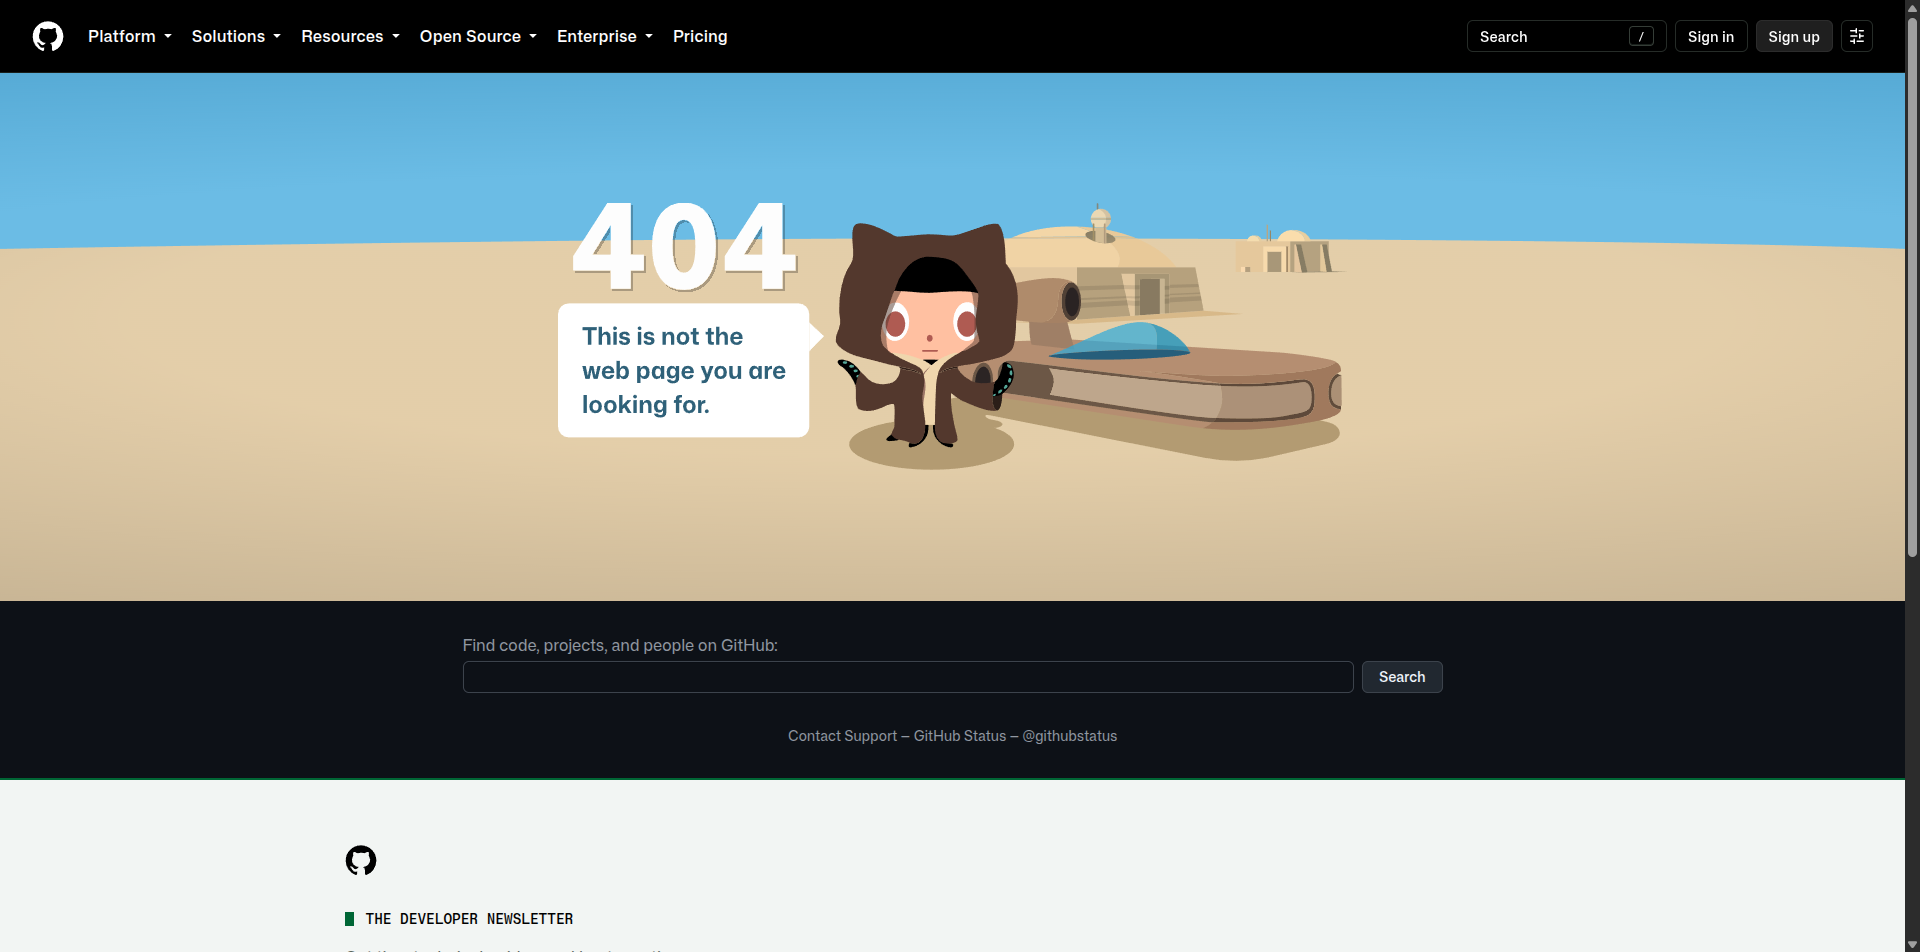
\includegraphics[width=0.95\textwidth]{images/ss-02-branch-protection.png}}
    \caption{Pengaturan Branch Protection Rules untuk cabang \texttt{main} dan \texttt{dev} pada repositori GitHub.}
    \label{fig:branch-protection}
\end{figure}

\subsection{Konfigurasi Workflow CI}
Alur kerja integrasi berkelanjutan didefinisikan pada berkas \texttt{.github/workflows/ci.yml}. Berkas ini mengonfigurasi dua pekerjaan pengujian yang berjalan secara independen:
\begin{enumerate}
    \item \textbf{Backend Test:} Mengatur lingkungan PHP 8.4, memasang dependensi Composer dari cache, menyiapkan basis data SQLite lokal, menjalankan migrasi, dan mengeksekusi \texttt{php artisan test}.
    \item \textbf{Frontend Build:} Mengatur lingkungan Node.js 20, memasang pustaka secara bersih menggunakan \texttt{npm ci}, dan memverifikasi kompilasi aset produksi melalui \texttt{npm run build}.
\end{enumerate}

\section{Continuous Deployment ke GHCR (CPMK 3)}
Soal nomor 4 mewajibkan penambahan pekerjaan penerapan (\textit{deploy job}) pada alur kerja GitHub Actions untuk mempublikasikan kontainer ke GitHub Container Registry (\texttt{ghcr.io}).

\subsection{Pemisahan Perilaku Eksekusi Deployment}
Sesuai butir soal 4.a, pekerjaan penerapan hanya boleh dijalankan saat terjadi peristiwa pengunggahan (\textit{push}) ke cabang \texttt{main}. Pada pengujian Pull Request atau pengunggahan ke cabang \texttt{dev}, pekerjaan \texttt{deploy} dilewati secara otomatis. Kondisi logika ini didefinisikan pada deklarasi pekerjaan:
\begin{lstlisting}[style=yamlstyle,caption={Potongan kondisi eksekusi job deploy pada ci.yml.}]
deploy:
  name: Deploy to GHCR
  needs: [backend-test, frontend-build]
  if: github.event_name == 'push' && github.ref == 'refs/heads/main'
  runs-on: ubuntu-latest
\end{lstlisting}

Bukti eksekusi alur kerja pada Pull Request cabang \texttt{dev} ditunjukkan pada Gambar \ref{fig:actions-pr-dev}, di mana pekerjaan \texttt{Backend Test} dan \texttt{Frontend Build} berhasil diselesaikan dengan warna hijau, sedangkan pekerjaan \texttt{Deploy to GHCR} dilewati (\textit{skipped}).

\begin{figure}[H]
    \centering
    \customfbox{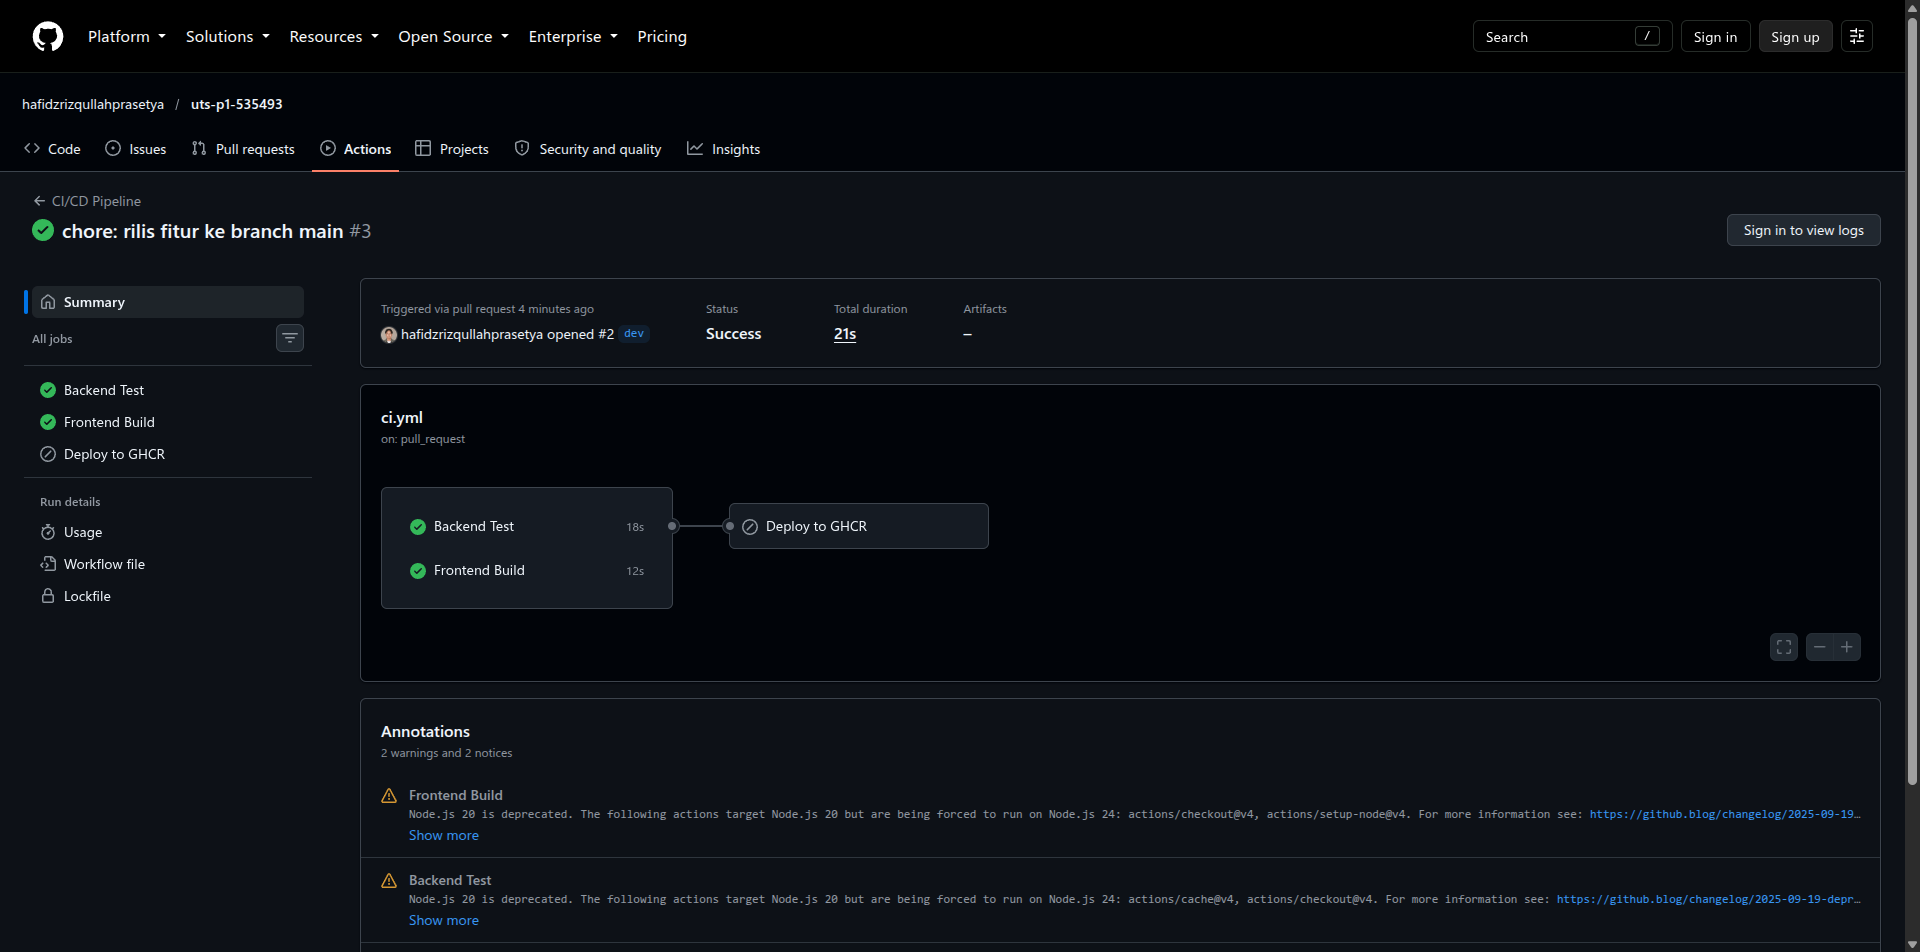
\includegraphics[width=0.95\textwidth]{images/ss-06-actions-pr-dev.png}}
    \caption{Riwayat alur kerja GitHub Actions pada Pull Request yang melewati tahap deployment.}
    \label{fig:actions-pr-dev}
\end{figure}

\subsection{Pengelolaan Kunci Rahasia dengan GitHub Secrets}
Sesuai butir soal 4.b, nilai konfigurasi sensitif seperti \texttt{APP\_KEY} dan \texttt{DB\_PASSWORD} disimpan pada menu \textit{Settings} $\rightarrow$ \textit{Secrets and variables} $\rightarrow$ \textit{Actions} di repositori GitHub. Variabel ini disuntikkan ke dalam proses pembangunan citra kontainer sebagai \textit{build-args} tanpa pernah ditulis secara terbuka di dalam repositori publik.

\subsection{Pemberian Tag Berdasarkan Commit SHA dan Registri GHCR}
Pekerjaan penerapan melakukan autentikasi ke registri \texttt{ghcr.io} menggunakan kredensial \texttt{GITHUB\_TOKEN} yang memiliki izin \texttt{packages: write}. Kontainer backend dan frontend dibangun dan diunggah dengan tag yang merujuk pada nomor commit penuh (\texttt{\$\{\{ github.sha \}\}}), bukan tag \texttt{latest}. Hal ini menjamin keterlacakan (\textit{traceability}) antara berkas artefak kontainer dan kode sumber yang menyusunnya.

Gambar \ref{fig:actions-main-deploy} memperlihatkan eksekusi alur kerja pada cabang \texttt{main} yang berhasil menyelesaikan ketiga pekerjaan secara berurutan dengan status hijau sempurna.

\begin{figure}[H]
    \centering
    \customfbox{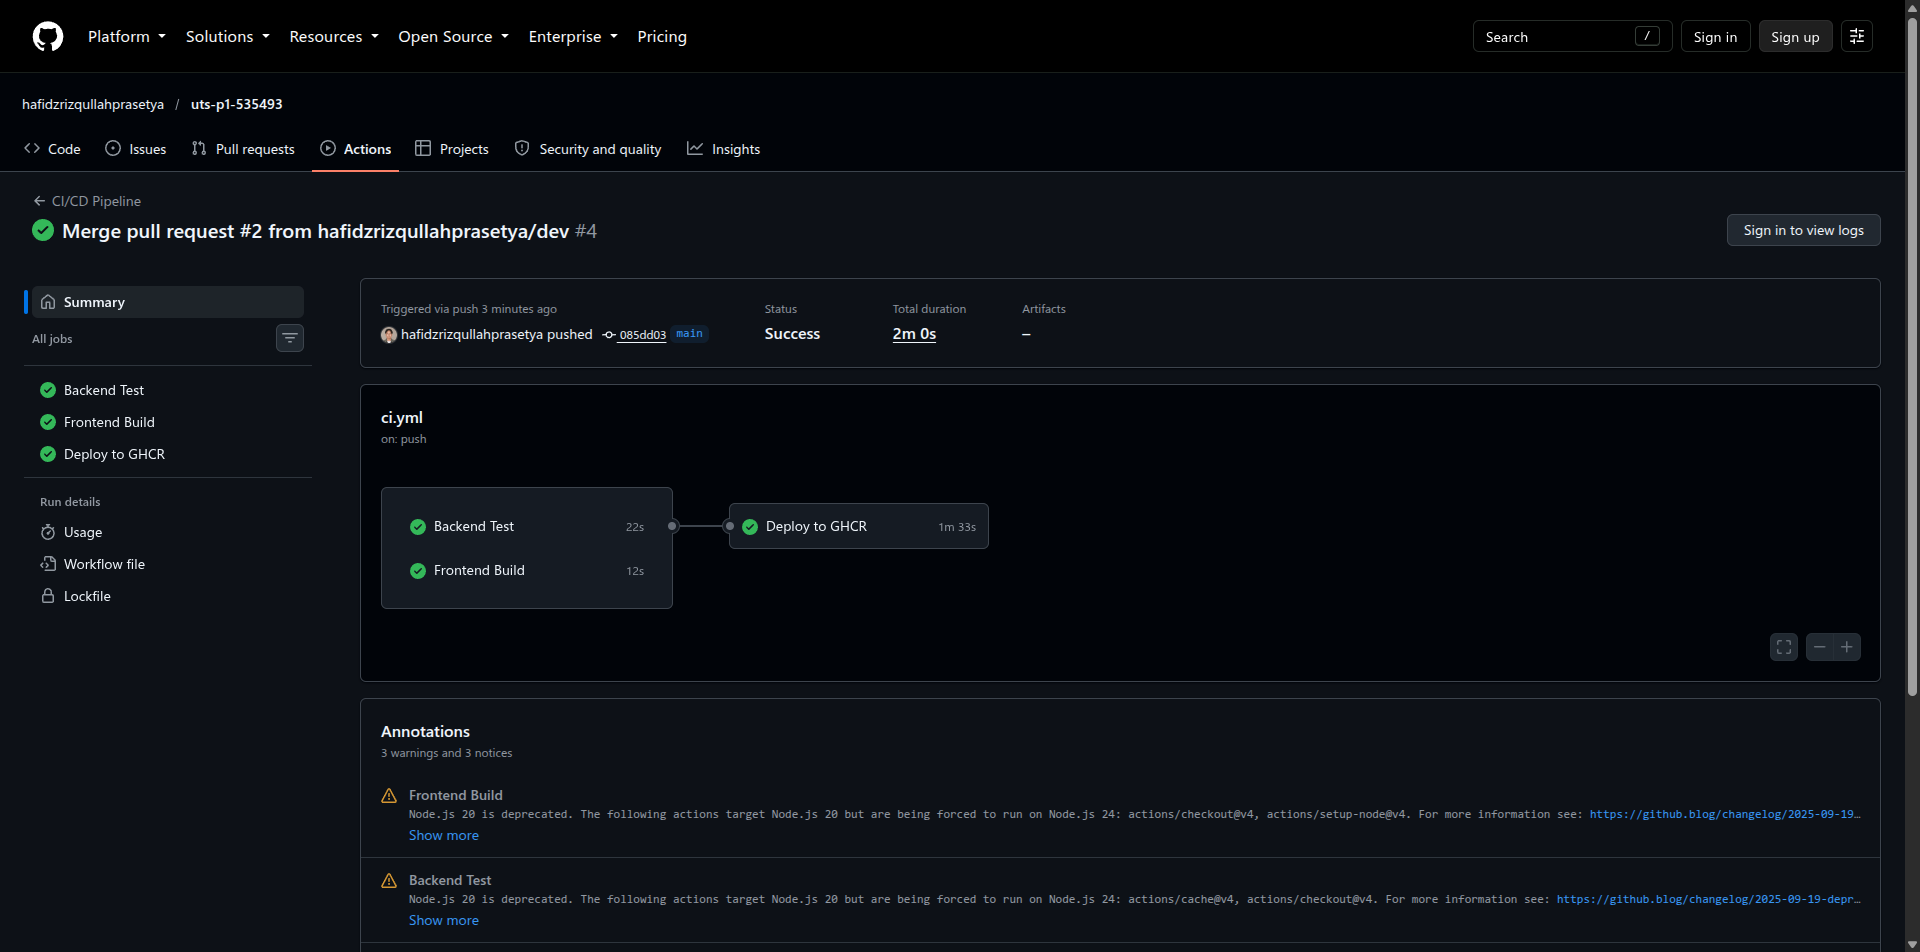
\includegraphics[width=0.95\textwidth]{images/ss-07-actions-main-deploy.png}}
    \caption{Eksekusi alur kerja CI/CD pada cabang \texttt{main} dengan tahap deploy yang berhasil diselesaikan.}
    \label{fig:actions-main-deploy}
\end{figure}

Seluruh riwayat alur kerja terangkum pada tab Actions repositori, sebagaimana disajikan pada Gambar \ref{fig:actions-tab}.

\begin{figure}[H]
    \centering
    \customfbox{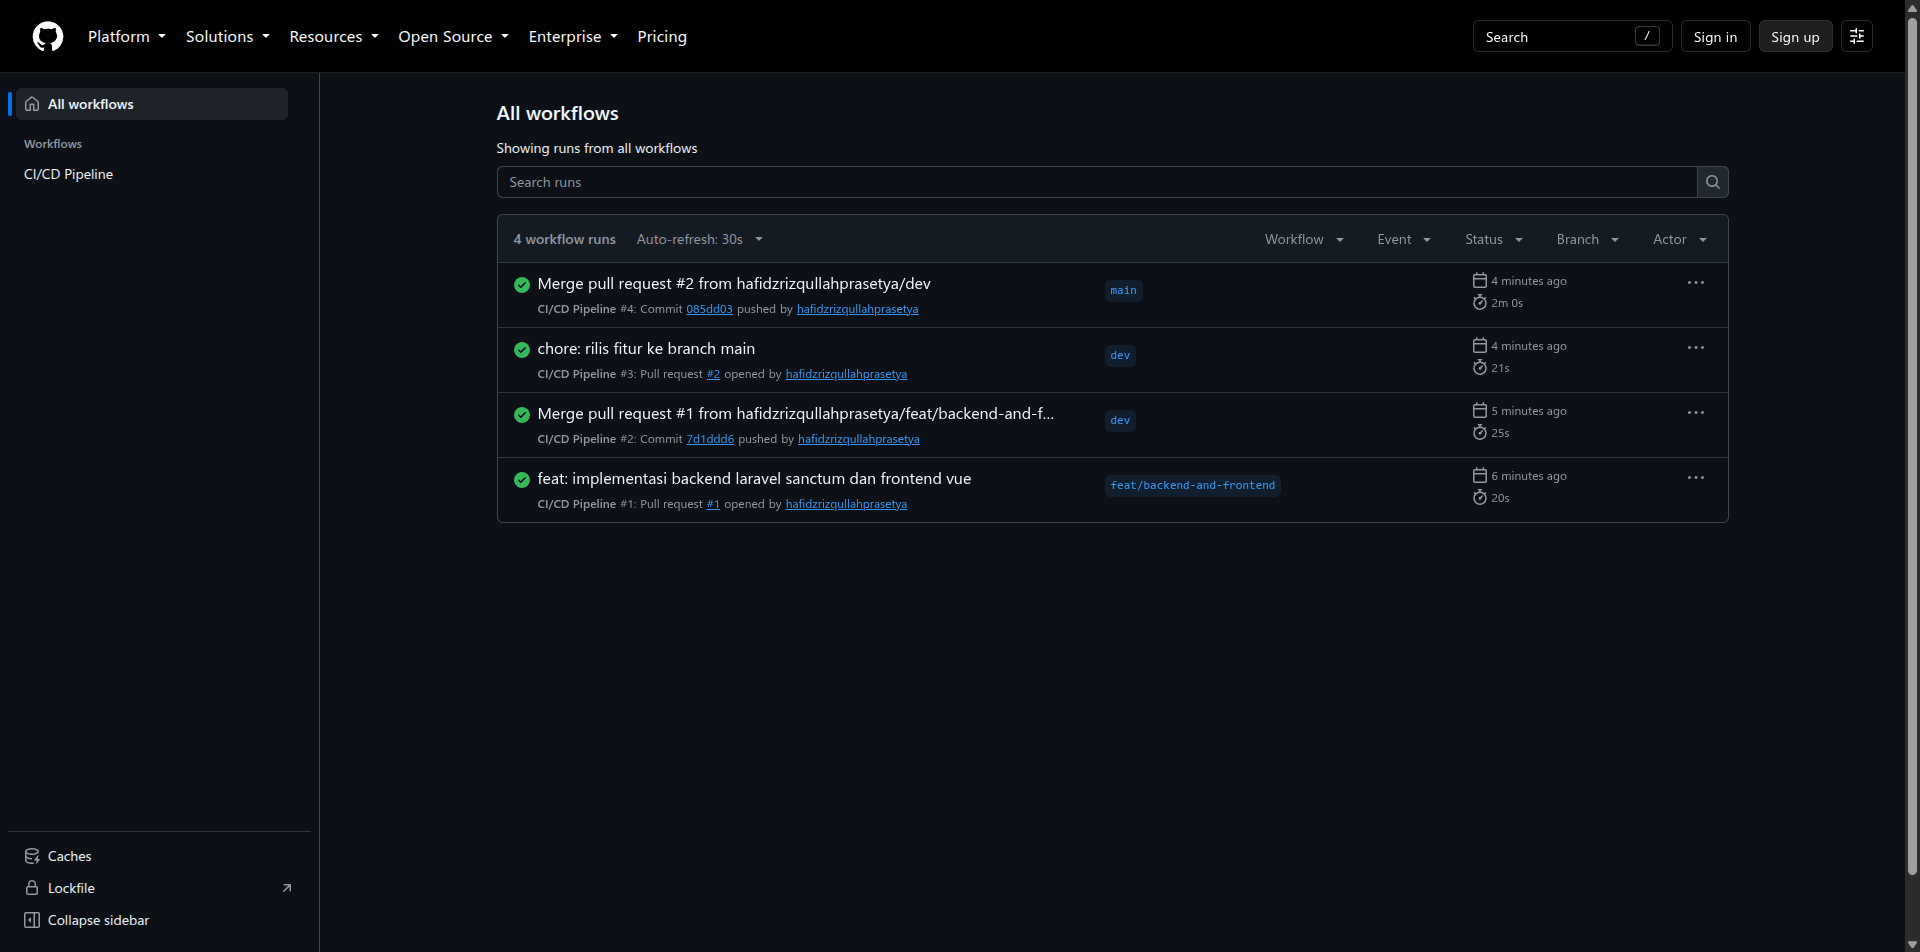
\includegraphics[width=0.95\textwidth]{images/ss-03-actions-tab.png}}
    \caption{Ringkasan riwayat eksekusi pipa CI/CD pada tab Actions repositori GitHub.}
    \label{fig:actions-tab}
\end{figure}

Hasil publikasi kedua citra kontainer pada GitHub Container Registry ditampilkan pada Gambar \ref{fig:packages-ghcr}. Kedua paket (\texttt{uts-p1-535493/backend} dan \texttt{uts-p1-535493/frontend}) terdaftar di bawah namespace repositori dan siap diunduh untuk kebutuhan orkestrasi peladen.

\begin{figure}[H]
    \centering
    \customfbox{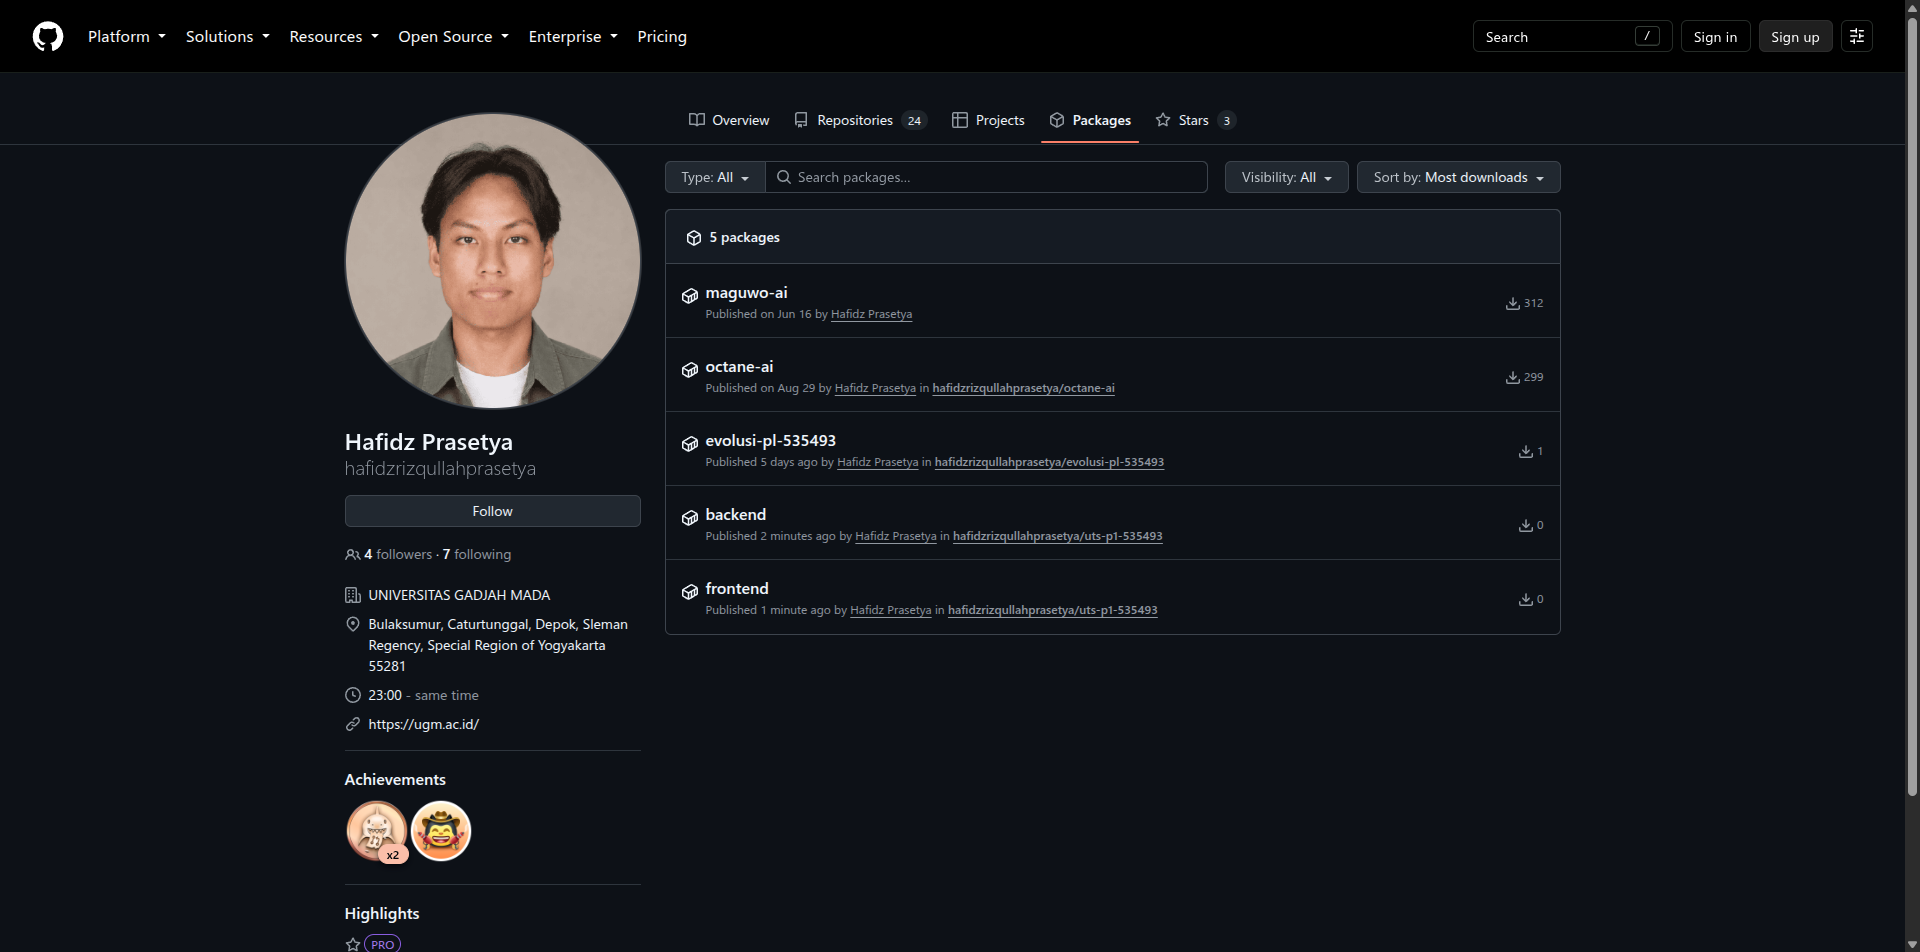
\includegraphics[width=0.95\textwidth]{images/ss-08-packages-ghcr.png}}
    \caption{Halaman registri paket GitHub Container Registry memuat citra backend dan frontend.}
    \label{fig:packages-ghcr}
\end{figure}

\section{Penyusunan Dockerfile Backend dan Frontend (CPMK 4 dan 5)}
Soal nomor 5 menuntut pembuatan berkas \textit{Dockerfile} untuk backend dan frontend dengan standar optimasi kontainerisasi industri.

\subsection{Dockerfile Backend dengan Optimasi Layer Caching}
Berkas \texttt{backend/Dockerfile} menggunakan citra dasar resmi \texttt{php:8.4-cli-alpine} yang eksplisit dan tidak menggunakan tag \texttt{latest}. Untuk mengoptimalkan kinerja \textit{cache} lapisan Docker, berkas manifes dependensi \texttt{composer.json} dan \texttt{composer.lock} disalin terlebih dahulu, diikuti eksekusi instalasi pustaka Composer tanpa skrip pengembang. Kode sumber aplikasi baru disalin pada lapisan berikutnya, seperti disajikan pada Listing \ref{lst:dockerfile-backend}.

\begin{lstlisting}[style=dockerstyle,caption={Berkas backend/Dockerfile dengan optimasi Composer layer caching.},label={lst:dockerfile-backend}]
FROM php:8.4-cli-alpine

WORKDIR /var/www/html

RUN apk add --no-cache \
    curl git unzip libzip-dev sqlite-dev \
    libpng-dev oniguruma-dev libxml2-dev linux-headers \
    && docker-php-ext-install -j$(nproc) \
    pdo pdo_sqlite mbstring xml zip bcmath

COPY --from=composer:2.8 /usr/bin/composer /usr/bin/composer

# Optimasi Layer Cache: Salin manifes dependensi terlebih dahulu
COPY composer.json composer.lock ./
RUN composer install --no-dev --no-scripts --no-autoloader --prefer-dist

# Salin sisa kode sumber aplikasi
COPY . .

RUN composer dump-autoload --optimize \
    && cp -n .env.example .env || true \
    && touch database/database.sqlite \
    && php artisan key:generate --force \
    && chown -R www-data:www-data storage bootstrap/cache database

EXPOSE 8000
CMD ["php", "artisan", "serve", "--host=0.0.0.0", "--port=8000"]
\end{lstlisting}

\subsection{Dockerfile Frontend Multi-Stage Build}
Berkas \texttt{frontend/Dockerfile} mengimplementasikan teknik \textit{multi-stage build}. Pada tahap pertama (\texttt{builder}), citra menggunakan \texttt{node:20-alpine} untuk memasang dependensi dan membangun aset web produksi melalui \texttt{npm run build}. Pada tahap kedua, citra produksi menggunakan peladen \texttt{nginx:1.27-alpine}. Berkas hasil build dari direktori \texttt{/app/dist} disalin ke direktori publik Nginx (\texttt{/usr/share/nginx/html}), sedangkan direktori \texttt{node\_modules} ditinggalkan pada tahap pertama. Pendekatan ini menghasilkan citra kontainer akhir yang sangat ramping dan aman, sebagaimana dicantumkan pada Listing \ref{lst:dockerfile-frontend}.

\begin{lstlisting}[style=dockerstyle,caption={Berkas frontend/Dockerfile menggunakan teknik multi-stage build.},label={lst:dockerfile-frontend}]
# Stage 1: Lingkungan build Node.js
FROM node:20-alpine AS builder

WORKDIR /app
COPY package*.json ./
RUN npm ci

COPY . .
RUN npm run build

# Stage 2: Lingkungan produksi Nginx
FROM nginx:1.27-alpine

RUN rm -rf /usr/share/nginx/html/*
COPY nginx.conf /etc/nginx/conf.d/default.conf
COPY --from=builder /app/dist /usr/share/nginx/html

EXPOSE 80
CMD ["nginx", "-g", "daemon off;"]
\end{lstlisting}

\chapter{BAB IV\\KESIMPULAN}
\renewcommand{\thechapter}{4}

Berdasarkan seluruh rangkaian perancangan, implementasi, dan pengujian yang telah dilaksanakan pada pengerjaan Ujian Tengah Semester mata kuliah Konstruksi dan Evolusi Perangkat Lunak, dapat ditarik beberapa kesimpulan sebagai berikut:
\begin{enumerate}
    \item Layanan backend berbasis Laravel RESTful API berhasil dibangun dengan tema Sistem Manajemen Aset Laboratorium. Autentikasi berbasis token Laravel Sanctum berhasil memproteksi seluruh rute privat, dengan implementasi kode status HTTP standar (201 Created, 422 Unprocessable Content, 401 Unauthorized, dan 200 OK) yang terverifikasi melalui 13 pengujian otomatis berstatus lulus dan koleksi Postman yang lengkap (CPMK 1).
    \item Antarmuka frontend berbasis Vue.js 3 dan Axios berhasil mengintegrasikan alur login, persistensi token pada penyimpanan lokal, dan operasi CRUD aset secara reaktif. URL API berhasil dipisahkan dari logika komponen melalui konfigurasi variabel lingkungan \texttt{VITE\_API\_BASE\_URL} (CPMK 1).
    \item Repositori sistem telah dikelola secara terstruktur di GitHub pada repositori publik \texttt{uts-p1-535493} dengan strategi cabang \texttt{main}, \texttt{dev}, dan cabang fitur. Aturan \textit{Branch Protection Rules} berhasil ditegakkan untuk mewajibkan alur Pull Request dan kelulusan pengujian CI sebelum penggabungan kode diizinkan (CPMK 2).
    \item Jalur penerapan berkelanjutan (\textit{Continuous Deployment}) berhasil dikonfigurasi pada alur kerja GitHub Actions. Pekerjaan deploy berhasil dibatasi hanya untuk kejadian push ke cabang \texttt{main}, memanfaatkan GitHub Secrets untuk variabel sensitif, dan mempublikasikan citra kontainer ke GitHub Container Registry (\texttt{ghcr.io}) dengan tag nomor commit SHA (CPMK 3).
    \item Kontainerisasi sistem berhasil dioptimalkan melalui penyusunan \textit{Dockerfile backend} yang memanfaatkan \textit{layer caching} dependensi Composer, serta \textit{Dockerfile frontend} yang menerapkan arsitektur \textit{multi-stage build} berbasis Nginx tanpa menyertakan direktori \texttt{node\_modules} pada citra akhir (CPMK 4 dan CPMK 5).
\end{enumerate}

\begin{thebibliography}{99}
\bibitem{laravel-sanctum}
Laravel LLC, ``Laravel Sanctum - Light-weight authentication for SPAs and token APIs,'' 2026. [Daring]. Tersedia: \url{https://laravel.com/framework/docs/sanctum}. [Diakses: 16-Okt-2026].

\bibitem{vuejs}
Vue.js Core Team, ``Introduction to Vue.js - The Progressive JavaScript Framework,'' 2026. [Daring]. Tersedia: \url{https://vuejs.org/guide/introduction.html}. [Diakses: 16-Okt-2026].

\bibitem{axios}
Axios Contributors, ``Axios HTTP Client - Getting Started,'' 2026. [Daring]. Tersedia: \url{https://axios.rest/pages/getting-started/first-steps}. [Diakses: 16-Okt-2026].

\bibitem{github-actions}
GitHub Inc., ``Understanding GitHub Actions - Workflow Automation and CI/CD,'' 2026. [Daring]. Tersedia: \url{https://docs.github.com/en/actions/get-started/understand-github-actions}. [Diakses: 16-Okt-2026].

\bibitem{github-protection}
GitHub Inc., ``About Protected Branches and Pull Request Gates,'' 2026. [Daring]. Tersedia: \url{https://docs.github.com/en/repositories/configuring-branches-and-merges-in-your-repository/managing-protected-branches/about-protected-branches}. [Diakses: 16-Okt-2026].

\bibitem{ghcr}
GitHub Inc., ``Working with the GitHub Container Registry (GHCR),'' 2026. [Daring]. Tersedia: \url{https://docs.github.com/en/packages/working-with-a-github-packages-registry/working-with-the-container-registry}. [Diakses: 16-Okt-2026].

\bibitem{docker-multistage}
Docker Inc., ``Multi-stage Builds - Optimize Container Image Sizes and Security,'' 2026. [Daring]. Tersedia: \url{https://docs.docker.com/build/building/multi-stage/}. [Diakses: 16-Okt-2026].

\bibitem{nginx}
Nginx Inc., ``Nginx Beginner's Guide - Web Server Configuration for Static Applications,'' 2026. [Daring]. Tersedia: \url{https://nginx.org/en/docs/beginners_guide.html}. [Diakses: 16-Okt-2026].
\end{thebibliography}

\end{document}
